\section{Model}

The model follows a discrete timing and embeds 4 types of agents ; the households, the firms, the fiscal authority and the central bank. Households can be either unemployed or employed through a fixed-term or an open-ended contract. Three types of firms coexist. Perfectly competitive final good producers generate the homogenous good valued by households for consumption and investment. This final good producers aggregate the differentiated goods produced by the retailers. The latter retailers are monopolistically competitive and transform the homegeneous intermediate good into a differentiated retail good. Intermediate firms produce the associated intermediate good and experience perfect competition. These intermediate firms, which we will simply call firms in what follows, use labor as their only input. In the following subsections, I describe the behavior of these agents in more detail.

\subsection{Households}

Households are identical and constitute a continuum represented  by the interval $(0,1)$. Perfect pooling of revenues leads to an equal consumption for all households, as in \citet{merz1995search} and \citet{andolfatto1996business}. Households hold the firms, consume the homogeneous good produced by final good firms and save using one-period nominal bonds. They earn wages, unemployment benefits, interests on their savings and pay lump-sum taxes. As a result, the households' program boils down to

\begin{align*}
&\max_{\left\{c_t, B_{t+1} \right\}_{t=0}^{+\infty}} \mathbb{E}_0 \sum_{t = 0}^{+\infty} \beta^t u\left(c_t\right)\\
&\text{s.t} \quad c_t + \frac{B_{t+1}}{P_t} = R_{t-1} \frac{B_{t}}{P_t} + \overline{w_t^p}_t n_t^p + \overline{w_t^f} n_t^f + b u_t + \Pi_t - \tau_t
\end{align*}

$C_t$ marks down consumption.\footnote{I omit the subscript $i$ since all households share the same allocations for consumption and savings.} $B_{t}$ is the amount of nominal bond holdings at the beginning of period $t$, with the associated nominal interest rate $R_t$ between $t$ and $t+1$. $\overline{w_t^p}$, $\overline{w_t^f}$ and $\overline{w_t}$ are respectively the average real wages for permanent jobs, temporary jobs and all workers. $b$ denotes the unemployment benefits. $n_t^p = \int_{0}^{1} n_{i,t}^p di$ is the aggregate permanent employment and $n_t^f$ denotes its temporary counterpart. $u_t$ marks down the measure of unemployed households. Firms transfer their profits to households through $\Pi_t$, while the government taxes $\tau_t$ to finance the payment of unemployment benefits.

The first order conditions with respect to $c_t$ and $B_{t+1}$ lead to the following Euler equation

\begin{align}
&\lambda_t = \beta \mathbb{E}_t \left[ R_{t} \frac{P_t}{P_{t+1}} \lambda_{t+1} \right] \label{eq:euler_eq}\\
&\lambda_t = u' \left( c_t \right)\label{eq:def_um}
\end{align}

The resulting firms' discount factor is $\beta_{t,s} = \beta^{s-t} \lambda_s / \lambda_t$ since households own firms.

\subsection{Final good firms}

Final good firms are identical and compete to produce the good consumed by households. They use a Dixit-Stiglitz aggregator as technology to put together retail goods and produce $Y_t$

\begin{equation}
Y_t = \left( \int_{0}^{1} Y_{i,t}^{\frac{\epsilon_t - 1}{\epsilon_t}} di \right)^{\frac{\epsilon_t}{\epsilon_t} - 1} \label{con_fin}
\end{equation}

where $\epsilon_t$ is the elasticity of substitution between retail goods.

The firm takes as given the price of the retail goods $P_{i,t}$ and the price of the final good $P_t$ and maximizes its profits with respect to the components of its input $\left\{Y_{i,t}\right\}_{i\in(0,1)}$ under the constraint \eqref{con_fin}. Therefore, the program of the final good firm boils down to

\begin{align*}
&\max_{\left\{Y_{i,t}\right\}_{i\in[0,1]}} P_t Y_t - \int_{0}^{1} P_{i,t} Y_{i,t} di\\
&\text{subject to \eqref{con_fin}}
\end{align*}

The subsequent first order condition provides an expression for the demand of the retail good $i$

\begin{equation}
Y_{i,t} = \left( \frac{P_{i,t}}{P_t} \right)^{-\epsilon_t} Y_t \label{ret_dem}
\end{equation}

\subsection{Retailers}

Retailers buy goods from intermediate firms and sell the obtained production to final good producer\footnote{At this step, it is possible to introduce capital to extend the model.}. They are monopolistically competitive and lie on the interval $(0,1)$. Retailers accomplish the one-to-one transformation of the intermediate good into a retail good. Denoting $X_{i,t}$ the retailer $i$'s input in the intermediate good, the production technology writes

\begin{equation*}
Y_{i,t} = X_{i,t}
\end{equation*}

As a result, retailers face a marginal cost that equals the relative price of the intermediate good $\phi_t$. I assume that these firms face a staggered price adjustment à-la \citet{calvo1983staggered}.

\begin{align*}
P_{i,t} = \left\{ \begin{array}{ll}
P_{i,t-1} & \text{ with probability } \psi\\
P_{i,t}^* & \text{ with probability } 1-\psi\\
\end{array}
\right.
\end{align*}

A fraction $\psi$ of retailers is able to adjust its prices to the optimal value $P_{i,t}^*$, whereas the  remaining retailers stick to their former prices. There is no indexation of non-adjusted princes on inflation in this model. Therefore, the price-setting retail firm $i$ at period $t$ experiences the following program

\begin{align*}
&\max_{P_{i,t}^*} \mathbb{E}_{t} \sum_{T = t}^{+\infty} \beta_{t,T} \psi^{T-t} \left( \frac{P_{i,t}^*}{P_T} - \phi_{T} \right) Y_{i,T} \\
&\text{ subject to } Y_{i,T} = \left( \frac{P_{i,t}^*}{P_T} \right)^{-\epsilon_t} Y_T
\end{align*}

where $\beta_{t,s}$ is the retailer's discount factor on time $t$ for a unit of profit earned at time $s$. This leads to the following first order condition

\begin{equation}
\mathbb{E}_{t} \sum_{T = t}^{+\infty} \beta_{t,T} \psi^{T-t} P_T^{\epsilon_T} Y_T \left( \frac{P_{i,t}^*}{P_T} - \mu_T \phi_T \right) = 0 \label{eq:price_eq}
\end{equation}

where $\mu_t = \epsilon_t /(\epsilon_t-1)$ is a mark-up shock such that $log\left( \mu_t \right) = \left(1-\rho_\mu\right) log\left( \epsilon / (\epsilon - 1) \right) + \rho_\mu log \left( \mu_{t-1} \right) + \epsilon_t^{\mu}$, with $\epsilon_t^{\mu} \overset{iid}{\sim} \mathcal{N} \left(0, \sigma_\mu^2 \right)$.

\subsection{Intermediate good firms and the labor market}

I mainly rely on \citet{rion:halshs-02331887} as for the general shaping of the labor market, which relates intermediate-good firms and households. Workers can be either employed or unemployed and are identical. There is no on-the-job search, which implies that only unemployed workers search for a job. Intermediate good firms are in perfect competition, sell their output to retailers at price $\phi_t$ and use labor as input. They can employ one worker or maintain one vacancy. These firms also face an aggregate productivity shock $A_t$. $A_t$ follows the process $log\left(A_t\right) = (1-\rho_A) log\left(\overline{A}\right) + \rho_A log\left(A_{t-1}\right) + \epsilon_t^A$, with $\epsilon_t^A \overset{iid}{\sim} \mathcal{N} \left( 0, \sigma_A^2 \right)$. The number of firm-worker contacts per period is $m(e,v)$, where $e$ is the number of job-seekers and $v$ is the number of vacancies. A classic measure of the matching activity is the labor market tightness $\theta =  v/e$. The matching function $m$ has constant returns to scale, which enables the definition of the firm-worker meeting probability $p(\theta)$ on the job seekers' side and its counterpart $q(\theta)$ on the firms' side.

\begin{align*}
q &= \frac{m\left(e,v\right)}{v} = m \left( \theta^{-1}, 1\right)\\
p &= \frac{m\left(e,v\right)}{e} = m \left( 1, \theta\right) = \theta q(\theta)\\
\end{align*}

The workers' firm-worker meeting probability is increasing, whereas the firms' firm-worker meeting probability is decreasing. Note that these meeting probabilities are not the classic job-finding and vacancy-filling probabilities. Indeed, in this paper, a firm-worker meeting does not necessarily lead to a productive firm-worker association. When a firm and a worker meet at period $t$, the idiosyncratic productivity of the match $z_t$ is revealed. Importantly, I assume that this idiosyncratic productivity is i.i.d across time and drawn from a distribution with cdf $G$. This assumption departs from the framework of \citet{rion:halshs-02331887}, where the idiosyncratic productivity of matches is persistent. I reluctantly make this assumption for the sake of simplicity on behalf of realism. Indeed, persistent idiosyncratic shocks require to keep track of the whole distribution of idiosyncratic productivities. Since this paper is, as far as I know, the first to describe fluctuations in a dual labor market with an endogenous contractual choice at the hiring stage, I prefer to leave the potentially complex distributional mechanisms for future research.

I now describe the timing in the economy. Figure \ref{fig:timing} sums it up. At the beginning of the period, agents learn the value of shocks. According to these new information, firms manage their workforce ; they may lay off workers and post vacancies. Next, new matches are revealed. Importantly, a paired firm and worker may return to search if the revealed productivity of the match is disappointing. Moreover, workers fired in the current period are able to participate to the present meeting round. This assumption is important to avoid an underestimation of the labor market flows, especially when the length of one periods is long compared  with the average length of a job. Indeed, temporary jobs last 1.5 months on average in France \citep{dares062018}, which might become a problem when the model is estimated on a quarterly basis and the workers must stay unemployed at least one period to be able to find a job again. Then, production is carried out, firms pay for wages and firing costs. At this point, households consume, and so ends the period. 

\begin{figure}[H]
\begin{center}
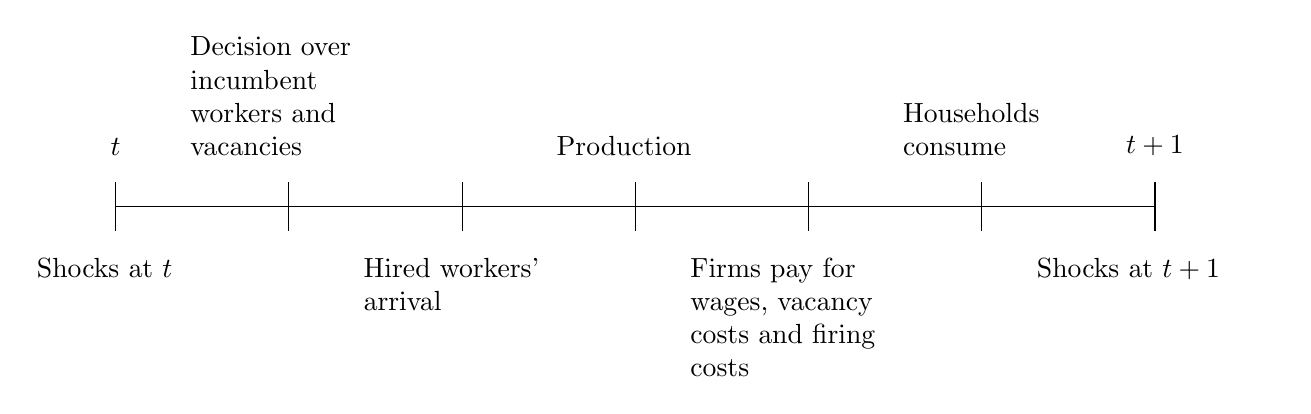
\begin{tikzpicture}[scale = 0.88]
%draw horizontal line
\draw (0cm,0cm) -- (15cm,0cm);
draw vertical lines
\foreach \x in {0, 2.5, 5, 7.5, 10, 12.5, 15}{
   \draw (\x,10pt) -- (\x,-10pt);
}
\draw (0,0) node[below=15pt, text width=2cm] {Shocks at $t$} node[above=15pt] {$t$};
\draw (2.5,0) node[above=15 pt, text width=2.5cm] {Decision over incumbent workers and vacancies};
\draw (5,0) node[below=15pt, text width=2.5cm] {Hired workers' arrival};
\draw (7.5,0) node[above=15pt, text width=2cm] {Production};
\draw (10,0) node[below=15pt, text width=3cm] {Firms pay for wages, vacancy costs and firing costs};
\draw (12.5,0) node[above=15pt, text width=2cm] {Households consume};
\draw (15,0) node[below=15pt, text width=3cm] {Shocks at $t+1$} node[above=15pt] {$t+1$};
\end{tikzpicture}
\end{center}
\label{fig:timing}
\caption{The timing of the economy}
\end{figure}

Now, I delineate the different possible situations on the labor market and the associated firms' and workers' surpluses.

\paragraph{Open-ended contracts}

A continuing open-ended contract delivers the wage $w_{t}^{p}$ and stipulates a firing tax $F_t = \phi_t A_t F$. On each period, an open-ended match may exogenously separate with probability $s$. In this case, the firing cost needs not to be paid. Otherwise, the firm chooses whether it keeps or lays off the worker regarding the idiosyncratic productivity of the match. An endogenous separation entails the payment of the firing cost. The firm's surplus with a continuing permanent match being increasing in $z_t$, I define the threshold $z_t^p$ below which paying the firing cost and dismissing the worker is preferrable. If I denote the firm's surplus with a continuing permanent match $J_t^p$ and the present discounted value of a vacancy $V_t$, I get the equation

\begin{align} \label{eq:def_jp}
J_t^p \left( z_{t} \right) = \phi_t A_t z_{t} - w_{t}^{p} \left( z_t \right) + \mathbb{E}_{t} \beta_{t,t+1} (1-s) \left\{ \int_{z_{t+1}^p}^{+\infty} J_{t+1}^{p} \left( z \right) dG(z) - G\left(z_{t+1}^p\right) F_{t+1} + s V_{t+1} \right\}
\end{align}

I denote $\xi_t$ the permanent job destruction probability, which verifies
 
\begin{equation} \label{eq:def_xi}
\xi_t = s+(1-s) G\left(z_t^p\right)
\end{equation}

A worker benefitting from a continuing permanent contract earns the wage $w_{t}^{p}$ and may either exogenously leave with probability $s$. If he does not, he faces a productivity shock and the match may split if the latter shock is adverse enough. As stated in the timing assumptions above, laid-off or quitting workers go back to the job seekers' pool immediately and are therefore eligible to participate to the current's period firm-worker meetings. I designate as $\widehat{U_t}$ the workers' associated present discounted value. Consequently, a continuing permanent worker's present discounted utility $W_t^p$ verifies

\begin{equation} \label{eq:def_wp}
W_t^p \left( z_t \right) = w_{t}^{p} \left( z_t \right) + \mathbb{E}_{t} \beta_{t,t+1} \left\{ (1-s) \int_{z_{t+1}^p}^{+\infty} W_{t+1}^p ( z ) dG(z) + \xi_{t+1} \widehat{U_{t+1}} \right\}
\end{equation}

New permanent matches stipulate different wages as their outside option does not include the payment of the firing cost in case of disagreement during the wage-bargaining process. Consequently, the surpluses of new open-ended matches involve the wage function $w_t^{0,p}$. After one-period, if there is no separation, a wage renegotiation occurs because idiosyncratic productivity changed. Firing costs now intervene in case of disagreement and the surpluses of continuing permanent contracts weigh in. Thus, the relevant functions of firm's and worker's surplus $J_{t}^{0,p}$ and $W_t^{0,p}$ follow

\begin{align} \label{eq:def_j0p} 
J_t^{0,p} \left( z_{t} \right) &= \phi_t A_t z_{t} - w_{t}^{0,p} \left( z_t \right) + \mathbb{E}_{t} \beta_{t,t+1} (1-s) \left\{ \int_{z_{t+1}^p}^{+\infty} J_{t+1}^{p} \left( z \right) dG(z) - G\left(z_{t+1}^p\right) F_{t+1} + s V_{t+1} \right\}\\
W_t^{0,p} \left( z_t \right) &= w_{t}^{0,p} \left( z_t \right) + \mathbb{E}_{t} \beta_{t,t+1} \left\{ (1-s) \int_{z_{t+1}^p}^{+\infty} W_{t+1}^p ( z ) dG(z) + \xi_{t+1} \widehat{U_{t+1}} \right\}
\end{align} 

\paragraph{Fixed-term contracts} A fixed-term contract stipulates the wage function $w_{i,t}^{f}$ and the exogenous destruction probability $\delta$\footnote{For an extensive discussion about the possibility of conversion into an open-contract contract at the expiry time and the endogenous choice of temporary jobs' durations, see \citet{rion:halshs-02331887}}. Importantly, it yields a lower productivity with respect to permanent contracts by factor $\rho < 1$. The latter assumption is an important departure with respect to \citet{rion:halshs-02331887}, where there is no productivity wedge between open-ended and fixed-term contracts \emph{a priori}. I need this assumption to preserve the properties derived in \citet{rion:halshs-02331887}, which essentially stem from the higher slope of open-ended matches' surplus with respect to the idiosyncratic productivity compared to fixed-term matches' surplus. In \citet{rion:halshs-02331887}, the latter is a consequence of the persistence of productivity shocks. Temporary matches experience a higher job destruction probability than permanent contracts while facing the same frequency of productivity shocks. As a result, temporary matches discount the current production at a higher rate than permanent ones, which reduces their slope with respect to the current productivity. Here, this mechanism does not intervene as idiosyncratic productivities of firm-worker pairs are i.i.d across time. 

A thought experiment provides better insights about the crucial nature of my assumption. For a given idiosyncratic productivity, if temporary and permanent contracts produced the same quantity of intermediate goods, there would be no room for labor market dualism at the equilibrium. One contract would be systematically preferred to the other at the hiring stage over the whole support of $G$. However, the assumption that temporary contracts are \emph{per se} less productive than permanent ones is not far-fetched in most cases. \citet{doi:10.1111/1467-9914.00212}, \citet{doi:10.1111/j.1467-9914.2007.00396.x}, \citet{Pfeifer2012} and \citet{Pfeifer2014} estimate that German and Spanish temporary workers experience wages 5 to 10 \% lower than their permanent counterparts. If wages reflect productivity, our assumption makes sense. Moreover, fixed-term positions are mainly filled by low-skilled or unexperienced workers \citep{fontaine2016cdd} and benefit less from on-the-job training \citep{doi:10.1111/1467-8543.00106,10.1162/154247604323068041,Albert2005,10.1093/esr/jcs011}. 

Firms value the immediate production net of the wage. As for the continuation value, it simply embeds the occurence or non-occurence of an exogenous separation shock. I denote $J_t^f$ the present discounted value of a temporary contract from the firm's point of view. 

\begin{equation} \label{eq:def_jf}
J_{t}^f \left( z_t \right) = \rho A_t z_t \phi_t - w_{t}^{f} \left( z_t \right) + \mathbb{E}_{t} \beta_{t,t+1} \left\{ \left( 1-\delta \right)  \int J_{t+1}^{f} \left( z \right) dG(z) + \delta V_{t+1} \right\}
\end{equation}

Temporary workers immediatly value their wage. In case of separation, they can participate to the currrent period's labor market trades. I designate as $W_t^f$ the worker's present discounted value of a temporary match, which follows

\begin{equation} \label{eq:def_wf}
W_{t}^f \left( z_t \right) = w_{t}^{f} \left( z_t \right) + \mathbb{E}_{t} \beta_{t,t+1} \left\{ \left( 1-\delta \right)  \int W_{t+1}^{f} \left( z \right) dG(z) + \delta \widehat{U_{t+1}} \right\}
\end{equation}

\paragraph{Vacancies} In opposition to most of the literature, the choice between a temporary and a permanent contract at the hiring step is explicitly embedded and in endogenous. When paired with a worker, firms can hire through a temporary contract or hire through a permanent contract. They are also able to return searching for a worker and get the chance to be matched with another one on the next period. The following equation bears witness of these possible options.

\begin{equation} \label{eq:def_v}
V_t = - \gamma + q \left( \theta_{t} \right) \int max \left[ J_{t}^{0,p} \left( z \right) , J_{t}^{f} \left( z \right) ,  E_{t} \beta_{t,t+1} V_{t+1} \right] dG(z)
\end{equation}

I assume that there is free entry for firms which post vacancies at the equilibrium.

\begin{equation}
V_t = 0 \label{eq:free_entry}
\end{equation}

The hiring regions of permanent contracts and temporary contracts are denoted $H_t^p$ and $H_t^f$, which are defined as follows

\begin{align}
H_t^p = \left\{ z_t : J_{t}^{0,p} \left( z_t \right) \geq \max\left[ J_{t}^{f} \left( z_t \right) ,  E_{t} \beta_{t,t+1} V_{t+1}  \right] \right\}\\
H_t^f = \left\{ z_t : J_{t}^{f} \left( z_t \right) \geq \max\left[ J_{t}^{0,p} \left( z_t \right) ,  E_{t} \beta_{t,t+1} V_{t+1}  \right] \right\}
\end{align}

Firms go back to searching for a worker when the drawn idiosyncratic productivity belongs to $H_t^u = \overline{H_t^p \cup H_t^f}$. As a result, the present discounted value of unemployment $U_t$ writes

\begin{align}  \label{eq:def_u}
U_t = b + \mathbb{E}_{t} \beta_{t,t+1} \widehat{U_{t+1}}
\end{align}

where $b$ is the unemployment benefit and $\widehat{U_t}$ is the present discounted value of the expected current period's trades on the labor market. It is the workers' outside option just before shocks hit. 

\begin{align} \label{eq:def_uhat}
\begin{split}
\widehat{U_t} &= p\left( \theta_t \right) \left( \int_{H_t^p} W_t^{0,p} (z) dG(z) + \int_{H_t^f} W_t^{f} (z) dG(z) + \left( \int_{H_t^u} dG(z) \right) U_{t} \right)\\
&+ \left( 1 - p\left( \theta_t \right) \right) U_{t}
\end{split}
\end{align}

\subsection{Wage bargaining}

I assume that wages are set each period through a Nash-bargaining process. Thus, denoting $\eta$ the worker's share of the surplus of the match, the sharing rules write

\begin{align}
&W_t^p \left( z_t \right) = \eta S_t^p \left( z_t \right) \label{eq:nash_p}\\
&W_t^{0,p} \left( z_t \right) = \eta S_t^{0,p} \left( z_t \right) \label{eq:nash_0p}\\
&W_t^f \left( z_t \right) = \eta S_t^f \left( z_t \right) \label{eq:nash_f}
\end{align}

where $S_t^p$ is the total surplus of a continuing permanent match, $S_t^{0,p}$ is the total surplus from a new permanent match and $S_t^{f}$ is the total surplus from a temporary match. These joint surpluses verify

\begin{align}
S_t^p \left( z_t \right) &= J_t^p \left( z_t \right) - \left( V_t - F_t \right) + W_t^p \left( z_t \right) - U_t \label{eq:def_sp}\\
S_t^{0,p} \left( z_t \right) &= J_t^{0,p} \left( z_t \right) - V_t + W_t^{0,p} \left( z_t \right) - U_t \label{eq:def_s0p}\\
S_t^{f} \left( z_t \right) &= J_t^{f} \left( z_t \right) - V_t + W_t^{f} \left( z_t \right) - U_t \label{eq:def_sf}
\end{align}

As intended, the continuing permanent worker's surplus includes the firing cost in case of endogenous separation. This bolsters his threat point in the Nash-bargaining process and pushes up his wage. The new permanent workers does not benefit from this effect since a failure in the bargaining process does not entail the payment of $F_t$.

Using the different definitions of the firms' and the workers' surpluses, the total surpluses write\footnote{Detailed calculations are available in Appendix \ref{sec:nb_surplus}}

\begin{align}
\begin{split} \label{eq:sp}
S_t^p \left( z_t \right) &= A_t z_t \phi_t - b + F_t - \mathbb{E}_t \beta_{t,t+1} (1-s) F_{t+1} - \mathbb{E}_t \beta_{t,t+1} \left( 1 - \xi_{t+1} \right) \frac{\eta \gamma \theta_{t+1}}{1-\eta}\\
&+ \mathbb{E}_t  \beta_{t,t+1} (1-s) A_{t+1} \phi_{t+1} \int_{z_{t+1}^p}^{+\infty} \left( 1 -  G(z) \right) dG(z)
\end{split}\\
S_t^{0,p} \left( z_t \right) &= S_t^p \left( z_t \right) - F_t \label{eq:s0p}\\
S_t^f \left( z_t \right) &= \rho A_t z_t \phi_t - b - \mathbb{E}_t \beta_{t,t+1} (1-\delta) \frac{\eta \gamma \theta_{t+1}}{1-\eta} + \rho \mathbb{E}_t \beta_{t,t+1} (1-\delta) A_{t+1} \phi_{t+1} \left( \mathbb{E}z - z_{t+1}^f \right) \label{eq:sf}
\end{align}

Using the expressions for the firms' surpluses with the expressions for the total surpluses above and the surplus sharing rules, the wages verify

\begin{align*}
w_t^p \left( z_t \right) &= \eta \left( A_t z_t \phi_t + F_t - E_t \beta_{t,t+1} (1-s) F_{t+1} + E_t \beta_{t,t+1} \left( 1-\xi_{t+1} \right) \gamma \theta_{t+1} \right) + (1-\eta) b\\
w_t^{0,p} \left( z_t \right) &= \eta \left( A_t z_t \phi_t - E_t \beta_{t,t+1} (1-s) F_{t+1} + E_t \beta_{t,t+1} \left( 1-\xi_{t+1} \right) \gamma \theta_{t+1} \right) + (1-\eta) b\\
w_t^f \left( z_t \right) &= \eta \left( \rho A_t z_t \phi_t + E_t \beta_{t,t+1} \left( 1-\delta \right) \gamma \theta_{t+1} \right) + (1-\eta) b\\
\end{align*}

The wage of the continuing permanent worker increases with the firing cost. The firing cost acts as a tax on separation but also as an upward force in the continuing permanent worker's threat point in the wage bargaining process. The new permanent worker is penalized with higher firing costs to compensate the future gains of wages in case of continuation. As usual in the Mortensen-Pissarides literature, the labor market tightness increases the outside option of the workers through the enlarged chances of finding a job and the wages raise.

In the case of Nash-bargaining, the hiring and firing decisions are efficient for both the worker and the firm. This may not be the case if wages are rigid.

\subsection{Job creation and job destruction}

The destruction of permanent contracts occurs when the surplus of a continuing match reaches zero. Thus, $z_t^p$ follows

\begin{align} \label{eq:def_zp}
S_t^p \left( z_t^p \right) = 0
\end{align}

Using \eqref{eq:sp}, this definition is equivalent to

\begin{align} \label{eq:zp}
\begin{split}
&A_t z_t^p \phi_t - b + F_t - \mathbb{E}_t \beta_{t,t+1} (1-s) F_{t+1} + \mathbb{E}_t  \beta_{t,t+1} (1-s) A_{t+1} \phi_{t+1} \int_{z_{t+1}^p}^{+\infty} \left( 1 -  G(z) \right) dG(z)\\
&= \mathbb{E}_t \beta_{t,t+1} \left( 1 - \xi_{t+1} \right) \frac{\eta \gamma \theta_{t+1}}{1-\eta}
\end{split}
\end{align}

At the hiring stage, temporary contracts become profitable when the productivity shock exceeds $z_t^f$ such that

\begin{align*}
S_t^{f} \left( z_t^f \right) &= 0
\end{align*}

Using \eqref{eq:sf}, $z_t^f$ verifies

\begin{align} \label{eq:zf}
\rho A_t z_t^f \phi_t - b + \rho \mathbb{E}_t \beta_{t,t+1} (1-\delta) A_{t+1} \phi_{t+1} \left( \mathbb{E}z - z_{t+1}^f \right) = \mathbb{E}_t \beta_{t,t+1} (1-\delta) \frac{\eta \gamma \theta_{t+1}}{1-\eta}
\end{align}

Analogously, new permanent contracts reach zero probitability at the threshold $z_t^c$, such that

\begin{equation*}
S_t^{0,p} \left( z_t^c \right) = 0
\end{equation*}

Since $\partial S_t^p / \partial z_t = A_t \phi_t$ and \eqref{eq:def_zp} is verified, one can rewrite the function $S_t^p$ as follows using an integration

\begin{equation} \label{eq:def_sp_lin}
S_t^p (z) = A_t \phi_t \left( z - z_t^p \right)
\end{equation}

In the same manner, the surplus associated with temporary contracts writes
\begin{equation} \label{eq:def_sf_lin}
S_t^f (z) = \rho A_t \phi_t \left( z - z_t^f \right)
\end{equation}

Consequently, \eqref{eq:def_sp_lin} provides a simple redefinition of $z_t^c$.

\begin{equation}
A_t \phi_t z_t^c = A_t \phi_t z_t^p + F_t \label{eq:zc}
\end{equation}

The job creation condition stems from the free-entry condition \eqref{eq:free_entry} and the Bellman equation defining the present discounted value of an unfilled vacancy \eqref{eq:def_v}. Using the Nash-sharing rules \eqref{eq:nash_0p}-\eqref{eq:nash_f}, the job creation condition becomes

\begin{align*}
\frac{\gamma}{(1-\eta) q\left( \theta_t \right)} = \int max \left[ S_t^{0,p} \left( z \right) , S_t^{f} \left( z \right), 0\right] dG(z)
\end{align*}



\begin{figure}[t]
\begin{center}
\begin{tikzpicture}

\newcommand\zp{0.62}
\newcommand\zf{1.08}
\newcommand\zs{1.28}
\newcommand\sigz{0.2}

\begin{axis}[
clip=false,
height = 10cm,
width = 10cm,
xlabel = $z$,
ylabel = {},	
xmin = exp(\sigz^2)-3*\sigz,
xmax = exp(\sigz^2)+4*\sigz,
ymin = 0.,
ymax = 2.25,
axis lines = middle,
legend pos= outer north east,
xtick = {\zp,\zf,\zs},
xticklabels={$z^p$,$z^f$,$z^*$}
]

\addplot[color = black,ultra thick,samples=1000,domain = 0.25:2.] { exp(-0.5*ln(x)^2/(0.2^2)) / (x*0.2*sqrt(2*pi))} ;
\addplot [color = black,thick,dashed]  coordinates { (\zp,0.) (\zp,{exp(-0.5*ln(\zp)^2/(0.2^2)) / (\zp*0.2*sqrt(2*pi))} ) };
\addplot [color = black,thick,dashed]  coordinates { (\zf,0.) (\zf,{exp(-0.5*ln(\zf)^2/(0.2^2)) / (\zf*0.2*sqrt(2*pi))} ) };
\addplot [color = black,thick,dashed]  coordinates { (\zs,0.) (\zs,{exp(-0.5*ln(\zs)^2/(0.2^2)) / (\zs*0.2*sqrt(2*pi))} ) };
\draw [thick,decoration={brace,mirror,amplitude = 10pt},decorate] (axis cs:{exp(\sigz^2)-3*\sigz},0.) -- (axis cs:\zp,0.) node[midway,below,yshift=-0.5cm] {Firing PC};
\draw [thick,decoration={brace,mirror,amplitude = 10pt},decorate] (axis cs:\zf,0.) -- (axis cs:\zs,0.) node[midway,below,yshift=-0.5cm] {Hiring TC};
\draw [thick,decoration={brace,mirror,amplitude = 10pt},decorate] (axis cs:\zs,0.) -- (axis cs:{exp(\sigz^2)+4*\sigz},0.) node[midway,below,yshift=-0.5cm] {Hiring PC};
\end{axis}

\end{tikzpicture}
\end{center}
\caption{The probability distribution function of idiosyncratic shocks and the location of thresholds}
\begin{flushleft}
\small The displayed pdf belongs to a log-Normal low with zero mean and standard deviation 0.2. \normalsize
\end{flushleft}
\label{fig:pdf}
\end{figure}

The economic mechanisms that follow are extensively described in \citet{rion:halshs-02331887}. The choice between temporary and permanent contracts lies in the comparison of joint surpluses across contracts. Interestingly, since $\partial S_t^{0,p} / \partial z_t = A_t \phi_t A_t > \rho A_t \phi_t = \partial S_t^{f} / \partial z_t$, there may exist a productivity threshold $z_t^*$ above which permanent contracts are preferable upon temporary ones. It will be the case in our calibration and estimation procedure. The discrimination between contracts is rooted in flexibility-productivity trade-off. Permanent contracts are more productive but are expensive during the downturns, whereas temporary contracts deliver a lower productivity but the associated workforce is more malleable because of the short stipulated durations. If job creation involves both temporary and permanent contracts, then Figure \ref{fig:pdf} sums up the hiring and firing policies.

Using the fact that $S_t^{0,p} \left( z_t^* \right) = S_t^{f} \left( z_t^* \right)$ with \eqref{eq:def_sp_lin} and \eqref{eq:def_sf_lin}, one finds that $z_t^*$ verifies

\begin{equation}
(1-\rho) z_t^* = z_t^c - \rho z_t^f \label{eq:zs}
\end{equation}

The behavior of the integrand of the job creation condition is summed up as follows

\begin{align*}
max \left[ S_t^{0,p} \left( z_t \right) , S_t^{f} \left( z_t \right), 0\right] = \left\{
\begin{array}{ll}
S_t^{0,p} \left( z_t \right) & \text{if } z_t \geq z_t^*\\
S_t^{f} \left( z_t \right) & \text{if } z_t^f \leq z_t \leq z_t^*\\
\end{array}
\right.
\end{align*}

Using the expressions of the derivatives of total surpluses with integration by parts, the job creation condition becomes

\begin{equation}
\frac{\gamma}{(1-\eta) A_t \phi_t q\left( \theta_t \right)} = \int_{z_t^*}^{+\infty} \left[ 1 - G(z) \right] dz + \rho \int_{z_t^f}^{z_t^*} \left[ 1 - G(z) \right] dz \label{eq:jc}
\end{equation}

\subsection{Fiscal and monetary policy}

In this framework, I assume that the government's role is to tax the households in order to provide for the unemployment benefits. The revenues from the firing tax get back to the government.  Therefore, the budget of the government is

\begin{equation}
\tau_t + (1-s) G\left( z_t^p \right) n_t^p F = b u_t + g_t
\end{equation}

where $g_t$ is the government expenditure and follows the AR(1) log-process $log\left(g_t\right) = \left(1-\rho_g\right) log\left(\overline{g}\right) + \rho_g log\left( g_{t-1} \right) + \epsilon_t^g$, $\epsilon_t^g \sim \mathcal{N} \left( 0, \sigma_g^2 \right)$.

The monetary policy is decided in accordance with a simple Taylor rule

\begin{equation}
log\left( R_{t} / R \right) = \rho_R log\left( R_{t-1} / R\right) + \left( 1 - \rho_R \right) \left[ \rho_{\pi} \mathbb{E}_t log \left( \frac{P_{t+1}}{P_t} \right) + \rho_y log\left(\frac{y_t}{y}\right) \right] + \epsilon_t^m \label{eq:taylor}
\end{equation}

where $y$ is the steady-state output and $\epsilon_t^m \overset{iid}{\sim} \mathcal{N} \left( 0, \sigma_m^2 \right)$.

Fixed-term contracts are known to behave as buffers in front of workload fluctuations, as Saint-Paul (1996) \cite{saint1996dual} documented. Thus, the case of indeterminacy in the Taylor rule and the subsequent appearance of sunspot equilibria may prove interesting. For the sake of simplicity, though, I shall restrain the present analysis to the determinate case with $\rho_{\pi} > 1$ and $\rho_y > 0$ and leave indeterminacy and its consequences on dual labor markets for future research.

\subsection{Market clearing conditions and the equilibrium}

This paragraph sums up the different conditions enabling an utter closing of the model. The employment values sum to the measure of households, namely 1.

\begin{equation}
n_t^p + n_t^f + u_t = 1
\end{equation}

where $n_t^p$ designates the measure of open-ended employees, $n_t^f$ the measure of fixed-term employees and $u_t$ unemployment.

The aggregate stock of job-seekers includes the formerly unemployed households and the new entrants in the unemployment pool from the current period.

\begin{equation}
e_t = u_{t-1} + \delta n_{t-1}^f + \xi_t n_{t-1}^p
\end{equation}

The labor market tightness is the ratio between aggregate number of vacancies $v_t = \int_{0}^{1} v_{i,t} di$ and the number of job seekers.

\begin{equation*}
\theta_t = \frac{v_t}{e_t}
\end{equation*}

The employment values evolve according to the following law of motions. The employment stocks drop by the job destruction flow and augment by the job creation flow.

\begin{align}
n_t^p &= \left( 1 - \xi_t \right) n_{t-1}^p + \mu_t^p e_t\\
n_t^f &= \left( 1 - \delta \right) n_{t-1}^f + \mu_t^f e_t
\end{align}

where $\mu_t^p = p\left( \theta_t \right) \left( 1- G\left( z_t^*\right)\right)$ and $\mu_t^f = p\left( \theta_t \right) \left( G\left( z_t^*\right)-G\left( z_t^f \right)\right)$ are the permanent and temporary job-finding rates respectively. The aggregate demand for final goods is

\begin{equation}
Y_t = c_t + g_t + \gamma v_t \label{eq:res_cons}
\end{equation}

The retailers face only one real marginal cost from the intermediate firms, which entails a unique equilibrium value for the optimal price-setting program, \emph{id est} $P_{i,t}^* = P_t^*$.

Meanwhile, the market clearing from intermediate goods writes

\begin{align*}
\int_{0}^{1} Y_{i,t} di &= A_t E_z \left[z \mid z \geq z_t^p \right] \left( 1 - \xi_t \right) n_{t-1}^p + \left( 1 - G\left( z_t^* \right)\right) q \left( \theta_t \right) v_t A_t E_z \left[z \mid z \geq z_t^* \right]\\
&+ \rho A_t \mathbb{E}_z \left[ z \right] \left( 1 - \delta \right) n_{t-1}^f + \rho \left( G\left( z_t^* \right) - G\left( z_t^f \right)\right) q \left( \theta_t \right) v_t A_t \mathbb{E}_z \left[z \mid z_t^* \geq z \geq z_t^f \right]
\end{align*}

Using the first order condition from the final good firm's program, I get

\begin{align}
\begin{split}
Y_t \Delta_t &= A_t E_z \left[z \mid z \geq z_t^p \right] \left( 1 - \xi_t \right) n_{t-1}^p + \left( 1 - G\left( z_t^* \right)\right) q \left( \theta_t \right) v_t A_t E_z \left[z \mid z \geq z_t^* \right]\\
&+ \rho A_t E_z \left[ z \right] \left( 1 - \delta \right) n_{t-1}^f + \rho \left( G\left( z_t^* \right) - G\left( z_t^f \right)\right) q \left( \theta_t \right) v_t A_t E_z \left[z \mid z_t^* \geq z \geq z_t^f \right] \label{eq:res_cons_int}
\end{split}
\end{align}

with $\Delta_t = \int_{0}^{1} \left( \frac{P_{i,t}}{P_t}\right)^{-\epsilon_t} di$ which measures price dispersion. \citet{yun1996nominal} demonstrated that the associated law of motion is

\begin{equation}
\Delta_t = (1-\psi) \left( \frac{P_t^*}{P_t} \right)^{-\epsilon_t} + \psi \left( \frac{P_t}{P_{t-1}} \right)^{\epsilon_t} \Delta_{t-1}
\end{equation}

while the price level follows

\begin{equation}
P_t = \left[ \psi P_{t-1}^{1-\epsilon_t} + (1-\psi) \left( P_t^* \right)^{1-\epsilon_t} \right]^{\frac{1}{1-\epsilon_t}} \label{eq:lm_price}
\end{equation}

Given the path of exogenous shocks $\left\{ \epsilon_t^A, \epsilon_t^\mu, \epsilon_t^g, \epsilon_t^m \right\}_{t=0}^{+\infty}$, laws of motions of exogenous shocks $\left\{ A_t, \mu_t , g_t \right\}_{t=0}^{+\infty}$ and initial values for the state variables $\left\{ i_{-1}, n_{-1}^p, n_{-1}^f, \Delta_{-1}, P_{-1} \right\}$, the equilibrium sums up into the set of endogenous variables $\left\{ i_t, c_t, Y_t, n_t^p, n_t^f, u_t, \Delta_t, z_t^p, z_t^c, z_t^f, z_t^*, \theta_t, \phi_t, v_t, P_t, P_t^* \right\}_{t=0}^{+\infty}$ pinned down by equations \eqref{eq:euler_eq}-\eqref{eq:def_um}, \eqref{eq:price_eq}, \eqref{eq:zp}-\eqref{eq:zf}, \eqref{eq:zs} and \eqref{eq:taylor}-\eqref{eq:lm_price}. 